\documentclass[11pt,openany]{article}

\usepackage{mathtools, commath}
% Packages for formatting
\usepackage[margin=1in]{geometry}
\usepackage{fancyhdr}
\usepackage{enumerate}
\usepackage{graphicx}
\usepackage{kotex}
\usepackage{arydshln} % Include this package
\usepackage{bbding}
\usepackage{amsmath}
\usepackage{amsthm}
\usepackage[dvipsnames,table]{xcolor}
\usepackage{amssymb, amsfonts}
\usepackage{wasysym}
\usepackage{footnote}
\usepackage{tablefootnote}
\usepackage{arydshln} % Include this package
% Fonts
\usepackage[T1]{fontenc}
\usepackage[utf8]{inputenc}
\usepackage{newpxtext,newpxmath}
\usepackage{sectsty}

% Define colors
\definecolor{TealBlue1}{HTML}{0077c2}
\definecolor{TealBlue2}{HTML}{00a5e6}
\definecolor{TealBlue3}{HTML}{b3e0ff}
\definecolor{TealBlue4}{HTML}{00293c}
\definecolor{TealBlue5}{HTML}{e6f7ff}

\definecolor{thmcolor}{RGB}{231, 76, 60}
\definecolor{defcolor}{RGB}{52, 152, 219}
\definecolor{lemcolor}{RGB}{155, 89, 182}
\definecolor{corcolor}{RGB}{46, 204, 113}
\definecolor{procolor}{RGB}{241, 196, 15}

\usepackage{color,soul}
\usepackage{soul}
\newcommand{\mathcolorbox}[2]{\colorbox{#1}{$\displaystyle #2$}}
\usepackage{cancel}
\newcommand\crossout[3][black]{\renewcommand\CancelColor{\color{#1}}\cancelto{#2}{#3}}
\newcommand\ncrossout[2][black]{\renewcommand\CancelColor{\color{#1}}\cancel{#2}}

\usepackage{hyperref}
\usepackage{booktabs}

% Chapter formatting
\definecolor{titleTealBlue}{RGB}{0,53,128}
\usepackage{titlesec}
\titleformat{\section}
{\normalfont\sffamily\Large\bfseries\color{titleTealBlue!100!gray}}{\thesection}{1em}{}
\titleformat{\subsection}
{\normalfont\sffamily\large\bfseries\color{titleTealBlue!50!gray}}{\thesubsection}{1em}{}

%Tcolorbox
\usepackage[most]{tcolorbox}
\usepackage{multirow}
\usepackage{multicol}

\usepackage[linesnumbered,ruled]{algorithm2e}
\usepackage{algpseudocode}
\usepackage{setspace}
\SetKwComment{Comment}{/* }{ */}
\SetKwProg{Fn}{Function}{:}{end}
\SetKw{End}{end}
\SetKw{DownTo}{downto}

% Define a new environment for algorithms without line numbers
\newenvironment{algorithm2}[1][]{
	% Save the current state of the algorithm counter
	\newcounter{tempCounter}
	\setcounter{tempCounter}{\value{algocf}}
	% redefine the algorithm numbering (remove prefix)
	\renewcommand{\thealgocf}{}
	\begin{algorithm}
	}{
	\end{algorithm}
	% Restore the algorithm counter state
	\setcounter{algocf}{\value{tempCounter}}
}

\usepackage{adjustbox}
% Header and footer formatting
\pagestyle{fancy}
\fancyhead{}
\fancyhf{}
\rhead{\textcolor{TealBlue2}{\large\textbf{기대수(기초부터 대학원 수학까지 시리즈) 3기}}}%\rule{3cm}{0.4pt}}
\lhead{\textcolor{TealBlue2}{\large\textbf{수학의 즐거움, Enjoying Math}}}
% Define footer
%\newcommand{\footer}[1]{
%\begin{flushright}
%	\vspace{2em}
%	\includegraphics[width=2.5cm]{school_logo.jpg} \\
%	\vspace{1em}
%	\textcolor{TealBlue2}{\small\textbf{#1}}
%\end{flushright}
%}
%\rfoot{\large Department of Information Security, Cryptogrphy and Mathematics, Kookmin Uni.\includegraphics[height=1.5cm]{school_logo.jpg}}
\fancyfoot{}
\fancyfoot[C]{-\thepage-}

\usepackage{tcolorbox}
\tcbset{colback=white, arc=5pt}

\definecolor{axiomcolor}{HTML}{a88bfa}
\definecolor{defcolor}{RGB}{52, 152, 219}
\definecolor{procolor}{RGB}{241, 196, 15}
\definecolor{thmcolor}{RGB}{231, 76, 60}
\definecolor{lemcolor}{RGB}{155, 89, 182}
\definecolor{corcolor}{RGB}{46, 204, 113}
\definecolor{execolor}{RGB}{90, 128, 127}

% Define a new command for the custom tcolorbox
\newcommand{\axiombox}[2][]{%
	\begin{tcolorbox}[colframe=axiomcolor, title={\color{white}\bfseries #1}]
		#2
	\end{tcolorbox}
}

\newcommand{\defbox}[2][]{%
	\begin{tcolorbox}[colframe=defcolor, title={\color{white}\bfseries #1}]
		#2
	\end{tcolorbox}
}

\newcommand{\lembox}[2][]{%
	\begin{tcolorbox}[colframe=lemcolor, title={\color{white}\bfseries #1}]
		#2
	\end{tcolorbox}
}

\newcommand{\probox}[2][]{%
	\begin{tcolorbox}[colframe=procolor, title={\color{white}\bfseries #1}]
		#2
	\end{tcolorbox}
}

\newcommand{\thmbox}[2][]{%
	\begin{tcolorbox}[colframe=thmcolor, title={\color{white}\bfseries #1}]
		#2
	\end{tcolorbox}
}

\newcommand{\corbox}[2][]{%
	\begin{tcolorbox}[colframe=corcolor, title={\color{white}\bfseries #1}]
		#2
	\end{tcolorbox}
}



\usepackage{amsthm}

% Define custom theorem styles
\newtheoremstyle{dotless} % Name of the style
{3pt} % Space above
{3pt} % Space below
{\itshape} % Body font
{} % Indent amount
{\bfseries} % Theorem head font
{} % Punctuation after theorem head
{2.5mm} % Space after theorem head
{} % Theorem head spec

\newtheoremstyle{definitionstyle} % Name of the style
{3pt} % Space above
{3pt} % Space below
{} % Body font
{} % Indent amount
{\bfseries} % Theorem head font
{.} % Punctuation after theorem head
{2.5mm} % Space after theorem head
{} % Theorem head spec

% Applying custom styles
\theoremstyle{dotless}
\newtheorem{theorem}{Theorem} % Theorem environment with section-wise numbering
\newtheorem{proposition}[theorem]{Proposition} % Theorem environment with section-wise numbering
\newtheorem{lemma}[theorem]{Lemma} % Lemma shares the counter with theorem
\newtheorem{corollary}[theorem]{Corollary} % Corollary shares the counter with theorem

\theoremstyle{definitionstyle}
\newtheorem*{observation}{\textcolor{Magenta}{Observation}}
\newtheorem{definition}{Definition} % Definition shares the counter with theorem
\newtheorem{example}{Example} % Example shares the counter with theorem
\newtheorem{exercise}{Exercise} % Example shares the counter with theorem
\newtheorem{remark}{Remark} % Remark shares the counter with theorem
\newtheorem*{note}{Note}

\newtheorem*{definition*}{Definition} % Definition shares the counter with theorem
\newtheorem*{example*}{Example} % Example shares the counter with theorem
\newtheorem*{exercise*}{\textcolor{violet}{Exercise}} % Example shares the counter with theorem
\newtheorem*{remark*}{Remark} % Remark shares the counter with theorem


\usepackage{tikz}
\usepackage{tikz-cd}
\usepackage{tikz-3dplot}
\usepackage{pgfplots}
\pgfplotsset{compat=newest} % Adjust to your version of pgfplots
\def\Circlearrowleft{\ensuremath{%
		\rotatebox[origin=c]{180}{$\circlearrowleft$}}}
\def\Circlearrowright{\ensuremath{%
		\rotatebox[origin=c]{180}{$\circlearrowright$}}}
\def\CircleArrowleft{\ensuremath{%
		\reflectbox{\rotatebox[origin=c]{180}{$\circlearrowleft$}}}}
\def\CircleArrowright{\ensuremath{%
		\reflectbox{\rotatebox[origin=c]{180}{$\circlearrowright$}}}}
\usetikzlibrary{
	3d, % For 3D drawing
	angles,
	arrows,
	arrows.meta,
	backgrounds,
	bending,
	calc,
	decorations.pathmorphing,
	decorations.pathreplacing,
	decorations.markings,
	fit,
	matrix,
	patterns,
	patterns.meta,
	positioning,
	quotes,
	shadows,
	shapes,
	shapes.geometric,
	tikzmark
}
\tikzset{
	% single mid‐path arrow
	mid arrow/.style={
		decoration={
			markings,
			mark=at position 0.5 with {\arrow{Stealth[scale=1.2]}}
		},
		postaction={decorate},
	},
	% style for field arrows
	field arrow/.style={
		-{Stealth[scale=1.0]},
		thick,
		blue!70!black,
	},
}
\newcommand{\ie}{\textnormal{i.e.}}
\newcommand{\rsa}{\mathsf{RSA}}
\newcommand{\rsacrt}{\mathsf{RSA}\textendash\mathsf{CRT}}
\newcommand{\inv}[1]{#1^{-1}}

%New Command
%\newcommand{\set}[1]{\left\{#1\right\}}
\newcommand{\N}{\mathbb{N}}
\newcommand{\Z}{\mathbb{Z}}
\newcommand{\Q}{\mathbb{Q}}
\newcommand{\R}{\mathbb{R}}
\newcommand{\cR}{\mathcal{R}}
\newcommand{\C}{\mathbb{C}}
\newcommand{\F}{\mathbb{F}}
\newcommand{\nbhd}{\mathcal{N}}
\newcommand{\Log}{\operatorname{Log}}
\newcommand{\Arg}{\operatorname{Arg}}
\newcommand{\pv}{\operatorname{P.V.}}

\newcommand{\of}[1]{\left( #1 \right)} 
%\newcommand{\abs}[1]{\left\lvert #1 \right\rvert}
%\newcommand{\norm}[1]{\left\| #1 \right\|}

\newcommand{\sol}{\textcolor{magenta}{\bf Sol}}
\newcommand{\conjugate}[1]{\overline{#1}}

\newcommand{\res}{\operatorname{res}}
\DeclareMathOperator*{\Res}{\operatorname{Res}}

%\renewcommand{\Re}{\operatorname{Re}}
%\renewcommand{\Im}{\operatorname{Im}}

\newcommand{\cyclic}[1]{\langle #1 \rangle}
\newcommand{\uniform}{\overset{\$}{\leftarrow}}
\newcommand{\xmark}{\textcolor{red}{\XSolidBrush}}
\newcommand{\vmark}{\textcolor{green!75!black}{\CheckmarkBold}}

\newcommand{\gen}[1]{\langle #1 \rangle}
\newcommand{\Gen}[1]{\left\langle #1 \right\rangle}

\newcommand{\img}[1]{\text{Img}(#1)}
\newcommand{\Img}[1]{\text{Img}\left(#1\right)}
\newcommand{\preimg}[1]{\text{Img}^{-1}(#1)}
\newcommand{\Preimg}[1]{\text{Img}^{-1}\left(#1\right)}

\newcommand{\relation}{\mathrel{\mathcal{R}}}
\newcommand{\injection}{\rightarrowtail}
\newcommand{\surjection}{\twoheadrightarrow}
\newcommand{\id}{\textnormal{id}}

\newcommand{\eqclass}[1]{\left[#1\right]}

% Define custom colors for O and X
\newcommand{\yes}{\textcolor{blue}{\bf \fullmoon}}
\newcommand{\no}{\textcolor{red}{\bf \texttimes}}

\DeclarePairedDelimiter\ceil{\lceil}{\rceil}
\DeclarePairedDelimiter\floor{\lfloor}{\rfloor}
%\renewcommand{\floor}[#1]{\lfloor #1\rfloor}
%\newcommand{\Floor}[#1]{\left\lfloor #1\right\rfloor}
%\newcommand{\ceil}[#1]{\lceil #1\rceil}
%\newcommand{\Ceil}[#1]{\left\lceil #1\right\rceil}

\newcommand{\topology}{\mathscr{T}}
\newcommand{\sequence}[1]{\langle #1\rangle}
\renewcommand{\vec}[1]{\mathbf{#1}}
\setstretch{1.25}

%\usepackage{background}
%\backgroundsetup{
%	scale=3,
%	color=gray!20,
%	opacity=0.3,
%	angle=45,
%	contents={\Huge \sffamily Ji, Yong-hyeon}
%}
\begin{document}
\pagenumbering{arabic}
\begin{center}
	\huge\textbf{Linear Algebra to Abstract Algebra}\\
	\vspace{0.5em}
	\large{Ji, Yong-hyeon}\\
%	\large{\ttfamily \url{https://github.com/Hacker-Code-J}}\\
	\vspace{0.5em}
	\normalsize{\today}\\
\end{center}

\noindent 
We cover the following topics in this note.
\begin{itemize}
	\item Subspace; Span
	\item Subgroup
	\item Homomorphism; Monomorphism; Epimorphism
	\item Isomorphism
	\item Kernel and Image
\end{itemize}
\hrule\vspace{12pt}
%\tableofcontents
\begin{center}
	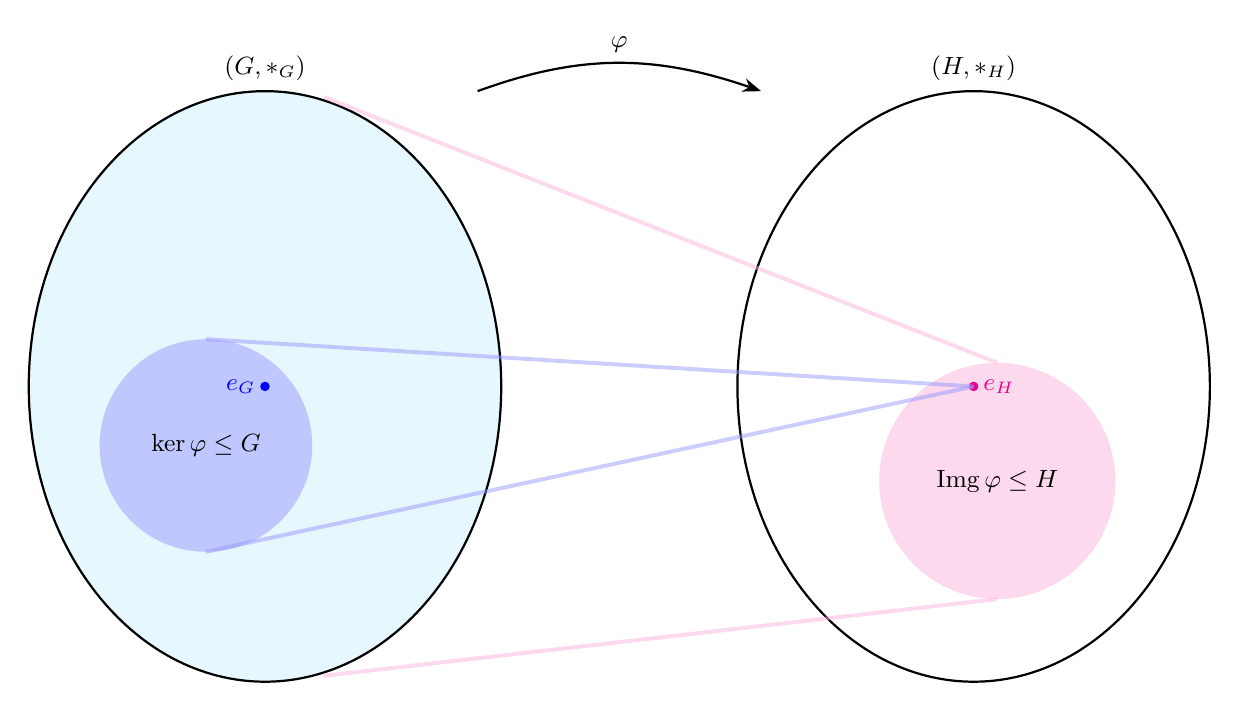
\begin{tikzpicture}[every node/.style={font=\small}, scale=1.5]
	% Ellipses
	\filldraw[cyan!10] (-3,0) ellipse (2 and 2.5);
	\draw[thick] (-3,0) ellipse (2 and 2.5) node[above=3.75cm] {$(G,\ast_G)$};
	\draw[thick] (3,0) ellipse (2 and 2.5) node[above=3.75cm] {$(H,\ast_H)$};
	
	% Arrows for homomorphism
	\draw[-Stealth, thick] (-1.2, 2.5) to[bend left=20] node[above] {$\varphi$} (1.2,2.5);
%	\node at (0,-3) {\textbf{Group Homomorphism}} ;
	
	% Kernel (inside G)
	\begin{scope}
		\clip (-3,0) ellipse (2 and 2.5);
		\fill[blue!40, opacity=0.5] (-3.5,-0.5) circle (0.9);
	\end{scope}
	\node at (-3.5,-0.5) {$\ker \varphi\leq G$};
	% Image (inside H)
	\begin{scope}
		\clip (3,0) ellipse (2 and 2.5);
		\fill[magenta!30, opacity=0.5] (3.2,-0.8) circle (1);
	\end{scope}
	\node at (3.2,-0.8) {$\operatorname{Img} \varphi\leq H$};
	
	\filldraw[blue] (-3,0) circle (1pt) node[left] {$e_G$};
	\filldraw[magenta] (3,0) circle (1pt) node[right] {$e_H$};
	
%	\draw[|->] (-2.85,0) to (2.85,0);
	
	\draw[magenta!30, line width=.5mm, opacity=0.5] (-3+.5,2.5-.05) to (3.2,.2);
	\draw[magenta!30, line width=.5mm, opacity=0.5] (-3+.5,-2.5+.05) to (3.2,-1.8);
	
	\draw[blue!40, line width=.5mm, opacity=0.5] (3,0) to (-3.5,.4);
	\draw[blue!40, line width=.5mm, opacity=0.5] (3,0) to (-3.5,-1.4);
\end{tikzpicture}
\end{center}

\newpage
\begin{note}[span]
Let $V$ be a vector space over a field $\F$, and let $S\subseteq V$. Recall that, for $n\in\N$, 
\begin{align*}
\Span(S):&=\set{\lambda_1\vec{v}_1+\lambda_2\vec{v}_2+\cdots+\lambda_n\vec{v}_n\mid \lambda_i\in\F,\; \vec{v}_i\in S\; \text{for all}\; i=1,2,\dots,n}\\
&=\set{\sum_{i=1}^n\lambda_i\vec{v}_i\; \bigg|\; \lambda_i\in\F,\; \vec{v}_i\in S\; \text{for all}\; 1\leq i\leq n}.
\end{align*}
\end{note}\vfill
\defbox[(Vector) Subspace]{\begin{definition*}
	Let $V$ be a vector space over a field $\F$, and let $U\subseteq V$. We write $
	\boxed{U\leq V}$ if $V$ is a \textbf{(vector) subspace} of $V$. That is, $U\leq V$ if and only if $U$ satisfy the following conditions: \begin{enumerate}[(i)]
		\item $\vec{0}_V\in U$;
		\item $\forall \vec{u},\tilde{\vec{u}}\in U$,\; $\vec{u}+\tilde{\vec{u}}\in U$;
		\item $\forall \vec{u}\in U$,\; $\forall \lambda\in\F$,\; $\lambda\vec{u}\in U$.
	\end{enumerate}
\end{definition*}}
\begin{remark*}
If $S\subseteq V$, then $\Span(S)\leq V$.
\begin{proof}
We must verify that $\Span(S)$ satisfies the three defining properties of a subspace of $V$: \begin{enumerate}[(i)]
	\item If $S=\varnothing$, by convention we define $\Span(\varnothing):=\set{\vec{0}_V}$. Let $S\neq\varnothing$. Choose any $\vec{v}\in S(\subseteq V)$ and take $n=1$ with the scalar $\lambda_1=0\in\F$. Then $\vec{0}_V=0\cdot\vec{v}\in\Span(S)$.
	\item Let $\vec{u},\tilde{\vec{u}}\in\Span(S)$, say, \[
	\vec{u}=\sum_{i=1}^{n}\lambda_i\vec{v}_i\quad\text{and}\quad\tilde{\vec{u}}=\sum_{j=1}^{m}\mu_j\tilde{\vec{v}}_j,
	\] where $n,m\in\N$, $\lambda_i,\mu_j\in\F$, and $\vec{v}_i,\tilde{\vec{v}}_j\in S$ for all indices $i,j$. Then \[
	\vec{u}+\tilde{\vec{u}}=\sum_{i=1}^{n}\lambda_i\vec{v}_i+\sum_{j=1}^{m}\mu_j\tilde{\vec{v}}_j=\overbrace{\underbrace{\lambda_1\vec{v}_1+\lambda_2\vec{v}_2+\cdots+\lambda_n\vec{v}_n}_{\text{$n$ terms}}+\underbrace{\mu_1\tilde{\vec{v}}_1+\mu_2\tilde{\vec{v}}_2+\cdots+\mu_m\tilde{\vec{v}}_m}_{\text{$m$ terms}}}^{\text{$n+m$ terms}}\in\Span(S).
	\]
	\item Let $\alpha\in\F$. Let $\vec{u}\in\Span(S)$, say, $\displaystyle\vec{u}=\sum_{i=1}^{n}\lambda_i\vec{v}_i,$  where $n\in\N$, $\lambda_i,\in\F$, and $\vec{v}_i\in S$ for each $1\leq i\leq n$. Then \[
	\alpha\vec{u}=\alpha\left(\sum_{i=1}^{n}\lambda_i\vec{v}_i\right)=\sum_{i=1}^{n}(\alpha\lambda_i)\vec{v}_i\overset{}{\in}\Span(S).
	\] since $\alpha\lambda_i\in\F$ for all $i=1,2,\dots,n$.
\end{enumerate}
\end{proof}
\end{remark*}

\newpage
\probox{\begin{proposition*}
Let $V$ be a vector space over a field $\F$, and let 
$S\subseteq V$. Then \begin{enumerate}[(1)]
	\item $S\subseteq\Span(S)\subseteq V$.
	\item If $U\leq V$ is any subspace of $V$ such that $S\subseteq U$, then $\Span(S)\subseteq U$.
\end{enumerate}
\end{proposition*}}
\begin{proof}
\ \begin{enumerate}[(1)]
	\item Let \( \vec{s} \in S \). Then, choosing \( n = 1 \) and \(\lambda_1 = 1 \in \F\), we have
		$\vec{s} = 1 \cdot \vec{s} \in \Span(S).$ Each element \( \vec{s} \in \Span(S) \) is of the form
		\[
		\vec{s} = \sum_{i=1}^n \lambda_i \vec{v}_i,
		\]
		where \( \vec{v}_i \in S \subseteq V \) and \( \lambda_i \in \F \). Since \( V \) is a vector space and is closed under finite linear combinations, it follows that $
		\vec{s} \in V.$
	\item Let \( U \le V \) and $S\subseteq U$. Let \( \vec{s} \in \Span(S) \). Then, there exist \( n \in \N \), scalars \( \lambda_1,\lambda_2, \dots, \lambda_n \in \F \), and vectors \( \vec{v}_1, \vec{v}_2 \dots, \vec{v}_n \in S\subseteq V \) such that
	\[
	\vec{s} = \sum_{i=1}^n \lambda_i \vec{v}_i\in\Span(S).
	\] Since \begin{itemize}
		\item $S\subseteq U$, \ie, $\vec{v}_i\in S\subseteq U$ for each $i=1,2,\dots,n$, and
		\item $U\leq V$, \ie, $\vec{u}+\tilde{\vec{u}}\in U$ and $\alpha\vec{u}\in U$ for any $\vec{u},\tilde{\vec{u}}\in U$,\; $\alpha\in\F$,
	\end{itemize} it follows that \[
\forall i\in\set{1,2,\dots,n},\; \lambda_i\vec{v}_i\in U\quad\text{and}\quad\vec{s}=\sum_{i=1}^n \lambda_i \vec{v}_i\in U.
	\]
\end{enumerate}
\end{proof}
\newpage
\probox{\begin{proposition*}
Let $V$ be a vector space over a field $\F$, and let $S\subseteq V$. Let $\mathcal{U}:=\set{U\leq V:S\subseteq U}.$ Then \[
\Span(S)=\bigcap_{U\in\mathcal{U}}U.
\] In other words, $\Span(S)$ is the smallest subspace of $V$ containing $S$.
\end{proposition*}}
\begin{proof}
We want to show that $\Span(S)=\bigcap_{U\in\mathcal{U}}U$.
\begin{itemize}
	\item[$(\subseteq)$] Let $\vec{u}\in\Span(S)$. By definition, there exists $n\in\N$, scalars $\lambda_1,\lambda_2,\dots,\lambda_n\in\F$, and vectors $\vec{v}_1,\vec{v}_2,\dots,\vec{v}_n\in S$ such that \[
	\vec{u}=\sum_{i=1}^n\lambda_i\vec{v}_i.
	\] Let $U\in\mathcal{U}$ be arbitrary. Since $S\subseteq U$ and $U\leq V$, it is closed under finite linear combinations: \[
	\sum_{i=1}^n\lambda_i\vec{v}_i\in U.
	\] Since $\forall U\in\mathcal{U},\; \vec{u}\in U\Leftrightarrow \vec{u}\in\bigcap_{U\in\mathcal{U}} U$, we obtain \[
	\vec{u}=\sum_{i=1}^n\lambda_i\vec{v}_i\in\bigcap_{U\in\mathcal{U}}U.
	\]
	\item[$(\supseteq)$] Since $S\subseteq\Span(S)$ and $\Span(S)\leq V$, we know $\Span(S)\in\mathcal{U}$. Let $\vec{u}\in\bigcap_{U\in\mathcal{U}}U$. Then \[
	\vec{u}\in\bigcap_{U\in\mathcal{U}}U\iff \forall U\in\mathcal{U},\; \vec{u}\in U\implies \vec{u}\in\Span(S).
	\]
\end{itemize} Hence, we conclude that $\Span(S)=\bigcap_{U\in\mathcal{U}}U$.
\end{proof}
\vfill
\defbox[Subgroup]{\begin{definition*}
	Let $G$ be a group. Let $H\subseteq G$. We say that $H$ is a \textbf{subgroup} of $G$, denoted by $H\leq G$, if and only if $H$ is itself a group \textcolor{gray!50}{(with the operation inherited from G)}.
\end{definition*}}
\begin{example*}
\ \begin{itemize}
	\item $(\Q,+)\leq(\R,+)$.
	\item $(\Q^\times,\times)\leq(\R^\times,\times)$.
\end{itemize}
\end{example*}

\probox[Subgroup Test]{\begin{proposition*}
Let $G$ be a group, and let $H\subseteq G$ with $H\neq\varnothing$. \begin{enumerate}[(1)]
	\item (2-step Test) \[
	H\leq G\iff \left(x,y\in H\implies xy\in H,\; x^{-1}\in H\right)
	\]
	\item (1-step Test) \[
	H\leq G\iff \left(x,y\in H\implies xy^{-1}\in H\right)
	\]
\end{enumerate}
\end{proposition*}}
\begin{proof}
We want to show that \[
\underbrace{H\leq G}_{\text{(a)}}\iff \underbrace{\left(x,y\in H\implies xy\in H,\; x^{-1}\in H\right)}_{\text{(b)}}\iff
\underbrace{\left(x,y\in H\implies xy^{-1}\in H\right)}_{\text{(c)}}
\] \vfill
\begin{itemize}
	\item[] $\left(\text{(a)}\Rightarrow\text{(b)}\right)$\; Let $H\leq G$. Let $x,y\in H$. Since every subgroup is closed under the group operation and taking inverses, we have \[
	xy\in H\quad\text{and}\quad x^{-1}\in H.
	\]\vfill
	\item[] $\left(\text{(b)}\Rightarrow\text{(c)}\right)$\; Let $x,y\in H$. Suppose that $xy\in H$ and $x^{-1}\in H.$ Clearly, $xy^{-1}\in H$.\vfill
	\item[] $\left(\text{(c)}\Rightarrow\text{(a)}\right)$\; Let $x,y\in H$. Suppose that \[
	xy^{-1}\in H.
	\] Since $H\neq\varnothing$, $\exists a\in H$, and so \[
	aa^{-1}\in H\implies e\in H.
	\] Since $x\in H$ and $e\in H$, we have \[
	ex^{-1}\in H\implies x^{-1}\in H.
	\] Then, since $x,y\in H$ and $y^{-1}\in H$, we obtain \[
	x(y^{-1})^{-1}\in H\implies xy\in H,
	\] \ie, $H$ is closed under binary operation on $G$.
\end{itemize}
\end{proof}

\newpage
\defbox[Subgroup Generated by $S$]{\begin{definition*}
	Let \( G \) be a group, and let \( S \subseteq G \).  
	The \textbf{subgroup of \( G \) generated by \( S \)}, denoted by
	$
	\langle S \rangle,$
	is defined as:
	\[
	\langle S \rangle \coloneqq \bigcap \{ H \le G : S \subseteq H \}=\bigcap_{S\subseteq H\leq G}H.
	\]
\end{definition*}}
\begin{exercise*}
Let $G$ be a group, and let $S\subseteq G$. Show that \(\langle S \rangle\) is the unique smallest subgroup of \( G \) containing \( S \).
\end{exercise*}
\begin{proof}[\sol]
	TBA
\end{proof}
\begin{exercise*}
Let $G$ be a group, and let $S\subseteq G$. Let $H_i\leq G$ for each $i\in I$. Show that \[
\bigcap_{i\in I} H_i\leq G.
\]
\end{exercise*}
\begin{proof}[\sol]
TBA
\end{proof}

\newpage
\probox[]{\begin{proposition*}
Let $(G,+)$ be an abelian group with identity $0_G$, and let $x,y\in G$. Then \begin{enumerate}[(1)]
	\item $\gen{x}=\set{nx:n\in\Z}$
	\item $\gen{x,y}=\set{nx+my:n,m\in\Z}$
\end{enumerate}
\end{proposition*}}
%\begin{remark*}
%	The notation $nx$ is defined to represent the $n$-fold sum of $x$ with itself when $n\geq 0$. We define the function \[
%	\fullfunction{f}{\textcolor{blue}{\Z}\times \textcolor{red}{G}}{\textcolor{red}{G}}{(n,x)}{nx}
%	\] by the following recursive rules: \begin{enumerate}
%		\item Base Case: $0x\coloneq0_G$.
%		\item Positive Integer: For $n\in\Z$ with $n\geq 1$, \[
%		nx\coloneq x+\underbrace{x+x+\cdots+x}_{\text{$n+(-1)=n-1$ times}},\quad\ie,\;\text{by induction}\;,\quad nx=x+(n-1)x.
%		\]
%		\item Negative Integer: For $n\in\Z$ with $n<0$, define \[
%		nx\coloneq \textcolor{red}{-}((\textcolor{blue}{-}n)x)
%		\]
%	\end{enumerate}
%	Here, for any $n\in Z$ with $n>0$, we have $(-n)x=x+(-n-1)x=2x+(-n-2)x= -(nx)$.
%\end{remark*}
\begin{proof}
	TBA
%\begin{enumerate}[(1)]
%	\item Define
%	\[
%	H_1 \coloneqq \{\, nx : n\in\mathbb{Z}\,\}.
%	\] We NTS that \(H_1\) is a subgroup of \(G\) and that \(H_1\) is the smallest subgroup containing \(x\).
%	\begin{enumerate}
%		\item (\(H_1\) is a subgroup of \(G\))
%		
%		Since $0\in\Z$ and $0x=0_G$, we have $0_G\in H_1$, \ie, $H_1\neq\varnothing$ Let $a,b\in H_1$. Then there exists $n,m\in\Z$ such that \[
%		a=nx\quad\text{and}\quad b=mx.
%		\] Then \[
%		a+(-b)=a+(-(mx)),
%		\] and since $n+(-m)\in\Z$, we have $a+(-b)\in H_1$.
%	\end{enumerate}
%	\item 
%\end{enumerate}
%
%(a) *\(H_1\) is a subgroup of \(G\):*  
%We verify the subgroup criteria:
%
%- **Nonemptiness:**  
%Since \(0\in\mathbb{Z}\) and \(0\cdot x = 0_G\), it follows that
%\[
%0_G\in H_1.
%\]
%
%- **Closure under Addition:**  
%Let \(n,m\in\mathbb{Z}\). Then
%\[
%n\cdot x + m\cdot x = (n+m)\cdot x \in H_1,
%\]
%because \(n+m\in\mathbb{Z}\).
%
%- **Closure under Inverses:**  
%For \(n\in\mathbb{Z}\), the additive inverse of \(n\cdot x\) is given by
%\[
%-(n\cdot x) = (-n)\cdot x \in H_1,
%\]
%since \(-n\in\mathbb{Z}\).
%
%Thus, \(H_1\le G\).
%
%(b) *\(H_1\) is the smallest subgroup containing \(x\):*  
%Let \(K\le G\) be any subgroup with \(x\in K\). Then, by the closure properties of \(K\),
%\[
%(\forall\, n\in\mathbb{Z})\quad n\cdot x \in K.
%\]
%Hence,
%\[
%H_1\subseteq K.
%\]
%By the definition of the subgroup generated by \(x\),
%\[
%\langle x\rangle = \bigcap\{ K\le G : x\in K\},
%\]
%it follows that
%\[
%\langle x\rangle \subseteq H_1.
%\]
%Conversely, since \(x\in H_1\) and \(H_1\) is a subgroup, we have
%\[
%\langle x\rangle \supseteq H_1.
%\]
%Therefore,
%\[
%\langle x\rangle = H_1 = \{\, n\cdot x : n\in\mathbb{Z}\,\}.
%\]
%
%2. **(Subgroup Generated by \(x\) and \(y\))**
%
%Define
%\[
%H_2 \coloneqq \{\, n\cdot x + m\cdot y : n,m\in\mathbb{Z}\,\}.
%\]
%
%We show that \(H_2\) is a subgroup of \(G\) and that \(H_2\) is the smallest subgroup containing both \(x\) and \(y\).
%
%(a) *\(H_2\) is a subgroup of \(G\):*  
%We check the subgroup criteria:
%
%- **Nonemptiness:**  
%With \(n=m=0\) we have
%\[
%0\cdot x + 0\cdot y = 0_G \in H_2.
%\]
%
%- **Closure under Addition:**  
%Let \(u,v\in H_2\) so that
%\[
%u = n\cdot x + m\cdot y \quad\text{and}\quad v = n'\cdot x + m'\cdot y,
%\]
%with \(n,m,n',m'\in\mathbb{Z}\). Then,
%\[
%u+v = (n+n')\cdot x + (m+m')\cdot y \in H_2,
%\]
%since \(n+n',\, m+m'\in\mathbb{Z}\).
%
%- **Closure under Inverses:**  
%For \(u = n\cdot x + m\cdot y \in H_2\),
%\[
%-u = (-n)\cdot x + (-m)\cdot y \in H_2,
%\]
%because \(-n,-m\in\mathbb{Z}\).
%
%Hence, \(H_2\le G\).
%
%(b) *\(H_2\) is the smallest subgroup containing \(x\) and \(y\):*  
%Let \(K\le G\) be any subgroup with \(x,y\in K\). Then by closure under the group operation,
%\[
%(\forall\, n,m\in\mathbb{Z})\quad n\cdot x + m\cdot y \in K.
%\]
%Therefore,
%\[
%H_2 \subseteq K.
%\]
%Since
%\[
%\langle x,y\rangle = \bigcap\{ K\le G : \{x,y\}\subseteq K\},
%\]
%it follows that
%\[
%\langle x,y\rangle \subseteq H_2.
%\]
%Conversely, as \(x,y\in H_2\) and \(H_2\) is a subgroup, we deduce that
%\[
%\langle x,y\rangle \supseteq H_2.
%\]
%Hence,
%\[
%\langle x,y\rangle = H_2 = \{\, n\cdot x + m\cdot y : n,m\in\mathbb{Z}\,\}.
%\]
%
%---
%
%**Conclusion.**  
%We have shown that if \((G,+)\) is an abelian group and \(x,y\in G\), then
%\[
%\langle x\rangle = \{\, n\cdot x : n\in\mathbb{Z}\,\} \quad\text{and}\quad \langle x,y\rangle = \{\, n\cdot x + m\cdot y : n,m\in\mathbb{Z}\,\}.
%\]
%This completes the formal proof.
%
%\[
%\quad\square
%\]
\end{proof}

\newpage
\begin{observation}
Let \begin{itemize}
	\item \((\mathbb{R}, +)\) is the additive group of real numbers, and 
	\item \((\mathbb{R}_{>0}, \cdot)\) is the multiplicative group of positive real numbers.
\end{itemize}
The \textbf{exponential function} is defined by \[
\fullfunction{\exp}{(\R,+)}{(\R_{>0},\cdot)}{x}{e^x}.
\] 
\begin{center}
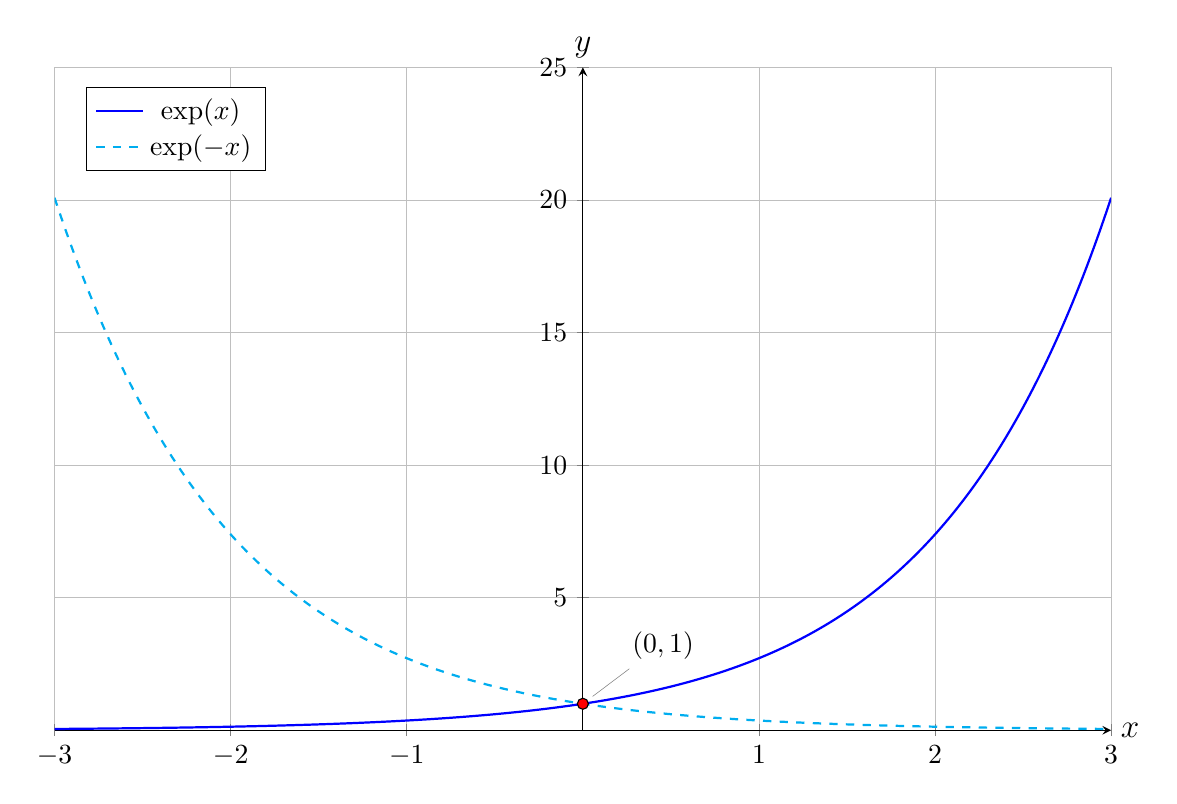
\begin{tikzpicture}
	\begin{axis}[
		width=15cm,
		height=10cm,
		axis lines=middle,
		xlabel={$x$},
		ylabel={$y$},
		xmin=-3, xmax=3,
		ymin=0, ymax=25,
		xtick={-3,-2,...,3},
		ytick={0,5,10,15,20,25},
		grid=both,
		major grid style={line width=.2pt,draw=gray!50},
		minor grid style={line width=.1pt,draw=gray!20},
		legend pos=north west,
		samples=300,
		domain=-3:3,
		xlabel style={font=\large, anchor=west},
		ylabel style={font=\large, anchor=south},
		]
		% Plot exp(x)
		\addplot [blue, thick] {exp(x)};
		% Plot exp(-x)
		\addplot [cyan, thick, dashed] {exp(-x)};
		\legend{\(\exp(x)\), \(\exp(-x)\)}
		% Mark the point (0,1) on both curves
		\addplot[only marks, mark=*, mark options={fill=red}] coordinates {(0,1)};
		\node[pin=45:{\(\,(0,1)\)}] at (axis cs:0,1) {};
	\end{axis}
\end{tikzpicture}
\end{center}
Then, \begin{enumerate}[(i)]
	\item $\exp(x+y)=e^{x+y}=e^{x}\cdot e^{y}=\exp(x)\cdot\exp(y)$;
	\item $\exp(0)=e^{0}=1$;
	\item $\exp(-x)=e^{-x}=(e^{x})^{-1}=(\exp(x))^{-1}$.
\end{enumerate}
\end{observation}
\newpage

\begin{observation}
Consider the exponential map \[
f \colon \mathbb{Z}_3 \to U_3,\quad f(x)=\exp\left(\frac{2\pi i}{3} x\right).
\] 
\begin{center}
\begin{tikzpicture}[scale=2, >=Stealth]
	% Axes
	\draw[->] (-1.2,0) -- (1.4,0) node[right] {$\text{Re}$};
	\draw[->] (0,-1.2) -- (0,1.2) node[above] {$\text{Im}$};
	
	% Unit circle
	\draw[gray!50, dashed] (0,0) circle(1);
	
	% Points
	\filldraw[blue] (1,0) circle (0.5pt) node[below right] {$f(0)=1$};
	\filldraw[blue] (-0.5,0.866) circle (0.5pt) node[above left] {$f(1)=\omega$};
	\filldraw[blue] (-0.5,-0.866) circle (0.5pt) node[below left] {$f(2)=\omega^2$};
	
	% Labels for origin
	\node at (0, -0.15) {0};
	
	% Optional: grid
%	 \draw[step=0.5cm, gray!20, very thin] (-1.5,-1.5) grid (1.5,1.5);
\end{tikzpicture}
\end{center}
Then $f$ is a group homomorphism from the additive group \((\mathbb{Z}_3, +)\) to the multiplicative group \( (U_3, \cdot) \) of the third roots of unity. Here, \begin{itemize}
	\item \(\mathbb{Z}_3=\{0,1,2\}\) with addition modulo 3
	\item $U_3=\{1,\,\omega,\,\omega^2\},\quad \text{with } \omega=\exp\Bigl(\frac{2\pi i}{3}\Bigr)$ which satisfies \(\omega^3=1\).
\end{itemize} The homomorphism property means that for all \(x,y\in\mathbb{Z}_3\) we have: \[
f(x+y)=f(x)f(y).
\]
\noindent
\begin{center}
\begin{minipage}{.49\textwidth}
(Addition Table in $\Z_3$) \[
\begin{array}{c|ccc}
	+ & 0 & 1 & 2 \\
	\hline
	0 & \cellcolor{magenta!50}0 & \cellcolor{cyan!50}1 & \cellcolor{orange!50}2 \\
	1 & \cellcolor{cyan!50}1 & \cellcolor{orange!50}2 & \cellcolor{magenta!50}0 \\
	2 & \cellcolor{orange!50}2 & \cellcolor{magenta!50}0 & \cellcolor{cyan!50}1
\end{array}
\]
\end{minipage}
\begin{minipage}{.49\textwidth}
(Multiplicative Table in $\Z_3$) \[
\begin{array}{c|ccc}
	\cdot & 0 & 1 & 2 \\
	\hline
	0 & \cellcolor{magenta!50}0 & \cellcolor{magenta!50}0 & \cellcolor{magenta!50}0 \\
	1 & \cellcolor{magenta!50}0 & \cellcolor{cyan!50}1 & \cellcolor{orange!50}2 \\
	2 & \cellcolor{magenta!50}0 & \cellcolor{orange!50}2 & \cellcolor{cyan!50}1
\end{array}
\]
\end{minipage}
\end{center}\vspace{10pt}
After applying the exponential map, the corresponding elements are:
\[
f(0)=1,\quad f(1)=\omega,\quad f(2)=\omega^2.
\]
Thus, the multiplication table is:
\[
\begin{array}{c|ccc}
	\cdot & 1 & \omega & \omega^2 \\
	\hline
	1 & \cellcolor{magenta!50}1 & \cellcolor{cyan!50}\omega & \cellcolor{orange!50}\omega^2 \\
	\omega & \cellcolor{cyan!50}\omega & \cellcolor{orange!50}\omega^2 & \cellcolor{magenta!50}1 \\
	\omega^2 & \cellcolor{orange!50}\omega^2 & \cellcolor{magenta!50}1 & \cellcolor{cyan!50}\omega
\end{array}\hspace{40pt}
\begin{array}{c|ccc}
	\cdot & f(0) & f(1) & f(2) \\
	\hline
	f(0) & \cellcolor{magenta!50}f(0) & \cellcolor{cyan!50}f(1) & \cellcolor{orange!50}f(2) \\
	f(1) & \cellcolor{cyan!50}f(1) & \cellcolor{orange!50}f(2) & \cellcolor{magenta!50}f(0) \\
	f(2) & \cellcolor{orange!50}f(2) & \cellcolor{magenta!50}f(0) & \cellcolor{cyan!50}f(1)
\end{array}
\]
\end{observation}

\newpage
\defbox[Homomorphism, Monomorphism, Epicmorphism, and Isomorphism]{\begin{definition*}
Let \( (G, \ast_G) \) and \( (H, \ast_H) \) be groups with identity elements \( e_G \) and \( e_H \), respectively. 
\begin{enumerate}[(1)]
	\item A function $\varphi : G \to H$
	is said to be a \textbf{group homomorphism} if and only if \[
	\varphi(x\ast_G y)=\varphi(x)\ast_H \varphi(y)\quad\text{for all}\;  x,y\in G.
	\]
	\item A group homomorphism \(\varphi: G \to H\) is called a \textbf{group monomorphism} iff it is injective.
	\item A group homomorphism \(\varphi: G \to H\) is called an \textbf{group epimorphism} iff it is surjective.
	\item A group homomorphism \(\varphi: G \to H\) is called an \textbf{group isomorphism} iff it is bijective.
\end{enumerate}
\end{definition*}}
\vfill
\defbox[Ring Homomorphism]{
\begin{definition*}
Let $(R, +_R, \cdot_R)$ and $(S, +_S, \cdot_S)$ be rings (with unity). A function \[
\varphi : (R, +_R, \cdot_R) \to (S, +_S, \cdot_S)
\] is called a \textbf{ring homomorphism} if \begin{enumerate}[(i)]
	\item $\varphi(a +_R b) = \varphi(a) +_S \varphi(b)$ for all $a,b\in R$\;
	\item $\varphi(a \cdot_R b) = \varphi(a) \cdot_S \varphi(b)$.
\end{enumerate} and, if the rings are unital, one additionally requires $
\varphi(1_R) = 1_S.$ It is immediate that this definition implies \(\varphi(0_R)=0_S\) since
\[
\varphi(0_R) = \varphi(0_R +_R 0_R) = \varphi(0_R) +_S \varphi(0_R).
\]
\end{definition*}
}
\vfill
\defbox[Module Homomorphism]{
\begin{definition*}
Let \(R\) be a ring and let \((M,+_M,\cdot_M)\) and \((N,+_N,\cdot_N)\) be \(R\)-modules. A function \[
f : (M,+_M,\cdot_M) \to (N,+_N,\cdot_N)
\] is an \textbf{\(R\)-module homomorphism} if the following hold: for all \(m_1,m_2\in M\) and for all \(r \in R\) 
\begin{enumerate}[(i)]
	\item $f(m_1+_Mm_2)= f(m_1)+_Nf(m_2)$\;
	\item $f(r\cdot_M m_1) = r\cdot_N f(m_1)$.
\end{enumerate}
%This definition ensures that \(f\) is compatible with both the additive group structure of \(M\) and the scalar multiplication by \(R\).
\end{definition*}
}

\newpage
\defbox[Linear Transformation (revised via Module Homomorphism)]{
\begin{definition*}
Let \(F\) be a field and let \(V\) and \(W\) be vector spaces over \(\F\); that is, \(V\) and \(W\) are \(F\)-modules. A function
\[
T : V \to W
\]
is called a \textbf{linear transformation} if the followings are satisfied: for every \(\vec{v}_1, \vec{v}_2 \in V\) and every scalar \(\lambda \in F\) \begin{enumerate}[(i)]
	\item $T(\vec{v}_1+\vec{v}_2) = T(\vec{v}_1) + T(\vec{v}_2)$;
	\item $T(\lambda \, \vec{v}_1) = \lambda\, T(\vec{v}_1)$.
\end{enumerate}
Thus, a linear transformation is precisely an \(\F\)-module homomorphism.	
\end{definition*}
}

\probox[Preservation of Identity and Inverses]{\begin{proposition*}
Let \((G, \cdot_G)\) and \((H, \cdot_H)\) be groups with respective identity elements \(e_G\) and \(e_H\), and let $\varphi : G \to H$ be a group homomorphism, that is,  \[
\varphi(a \cdot_G b) = \varphi(a) \cdot_H \varphi(b)\quad\text{for all}\; a,b\in G.
\] Then the following hold: \begin{enumerate}[(1)]
	\item \textbf{Preservation of Identity:}\quad $
	\varphi(e_G) = e_H.$
	\item \textbf{Preservation of Inverse:}\quad$
	\varphi\bigl(a^{-1}\bigr) = \bigl(\varphi(a)\bigr)^{-1}$ for all $a \in G$.
\end{enumerate}
\end{proposition*}}
\begin{proof}
	TBA
%*Proof Sketch:*  
%For (1), observe that
%\[
%\varphi(e_G) = \varphi(e_G \cdot_G e_G) = \varphi(e_G) \cdot_H \varphi(e_G),
%\]
%which, by the cancellation property in \(H\), implies \(\varphi(e_G) = e_H\). For (2), using (1) and the homomorphism property,
%\[
%\varphi(a) \cdot_H \varphi\bigl(a^{-1}\bigr) = \varphi(a \cdot_G a^{-1}) = \varphi(e_G) = e_H,
%\]
%so that \(\varphi\bigl(a^{-1}\bigr)\) is the inverse of \(\varphi(a)\).
\end{proof}

\newpage
\defbox[Kernel]{\begin{definition*}
Let \(\varphi : G \to H\) be a group homomorphism. The \textbf{kernel of \(\varphi\)} is the subset of \(G\) defined by
\[
\ker(\varphi) \coloneqq \{ g \in G : \varphi(g) = e_H \}.
\]
\end{definition*}}
\begin{remark*}
	The set \(\ker(\varphi)\) is a \st{normal} subgroup of \(G\).
	\begin{proof}
		TBA
	\end{proof}
\end{remark*}

\defbox[Image]{\begin{definition*}
Let \(\varphi : G \to H\) be a group homomorphism. The \textbf{image} of \(\varphi\) is the subset of \(H\) given by
\[
\operatorname{Img}(\varphi) \coloneqq \{ h \in H : \exists\, g \in G \text{ such that } \varphi(g) = h \}=\set{\varphi(g):g\in G}.
\]
\end{definition*}}
\begin{remark*}
	The set \(\operatorname{Img}(\varphi)\) forms a subgroup of \(H\).
	\begin{proof}
		TBA
	\end{proof}
\end{remark*}


\vfill
\begin{thebibliography}{9}
	\bibitem{linear_to_abstract_a}
	수학의 즐거움, Enjoying Math. ``수학 공부, 기초부터 대학원 수학까지, 18. 선형대수학에서 추상대수학으로 (a) 선형결합의 추상화'' YouTube Video, 24:25. Published 
	October 15, 2019. URL: \url{https://www.youtube.com/watch?v=zg63xXZYNM8&t=598s}.
	\bibitem{linear_to_abstract_b}
	수학의 즐거움, Enjoying Math. ``수학 공부, 기초부터 대학원 수학까지, 19. 선형대수학에서 추상대수학으로 (b) 대수적 구조를 보존하는 함수 algebraic homomorphisms'' YouTube Video, 25:21. Published 
	October 16, 2019. URL: \url{https://www.youtube.com/watch?v=9TtGaY5COlg&t=187s}.
\end{thebibliography}

\end{document}
